\documentclass[11pt]{article}
%Gummi|061|=)
\usepackage{graphicx}
\usepackage{subfig}
\title{\textbf{Image registration}}
\date{}
\begin{document}

\maketitle
\section{Rotation operations}
Given three vectors $u,v,w \in \mathbf{R}^3$, we have the following identity (it can be directly verified):
\begin{equation}
    u\times(v \times w) = (u^T w)v - (u^T v)w,
\end{equation}
in particular, for $u=v$:
\begin{equation}
    v\times(v \times w) = (v^T w)v - ||v||^2w.
\end{equation}
By defining the ``hat'' transformation for a vector $v=(v_0, v_1, v_2)$ to a skew symmetric matrix:
\begin{equation}
    \hat{v} = \left[\begin{array}{ccc}
        0 & -v_2 & v_1 \\
        v_2 & 0 & -v_0 \\
        -v_1 & v_0 & 0
    \end{array}\right],
\end{equation}
we have the following property:
\begin{equation}
    \hat{v}w = v \times w
\end{equation}
where $\hat{v}w$ is the usual matrix-vector product. Now, let's fix a vector $v\in \mathbf{R}^{3}$, then, \textbf{for every} vector $w\in \mathbf{R}^{3}$ we have
\begin{equation}
    \hat{v}^{3}w = \hat{v}(v\times (v \times w)) = \hat{v}(v^T w - ||v||^2 w) = (v^T w)\hat{v}w - ||v||^{2}\hat{v}w = - ||v||^{2}\hat{v}w
\end{equation}
because $\hat{v}v=v \times v = 0$. Therefore, $\hat{v}^{3} = -||v||^{2}\hat{v}$. Now:
\begin{equation}
    \hat{v}^{4} = \hat{v}^{3}\hat{v} = -||v||^{2}\hat{v}^{2}
\end{equation}
and interestingly, all powers can be written as scalar factors of $\hat{v}$ and $\hat{v}^{2}$ (alternating signs):
\begin{equation}
    \begin{array}{l}
        \hat{v}^{2n+1} = (-1)^{n}||v||^{2n}\hat{v}\\
        \hat{v}^{2n+2} = (-1)^{n}||v||^{2n}\hat{v}^{2}
    \end{array}.
\end{equation}
This allows us to easily compute the exponential of any skew symmetric matrix of the form $\hat{v}$ by splitting the powers of the Taylor expansion into odd and even powers:
\begin{equation}
    \exp(\hat{v})=\sum_{k=0}^{\infty}\frac{1}{k!}\hat{v}^{k} = I + \left[\sum_{k=0}^{\infty}\frac{(-1)^{k}||v||^{2k}}{(2k+1)!}\right]\hat{v}+
    \left[\sum_{k=0}^{\infty}\frac{(-1)^{k}||v||^{2k}}{(2k+2)!}\right]\hat{v}^{2}
\end{equation}
\begin{equation}
    \exp(\hat{v})=I + \frac{\sin{||v||}}{||v||}\hat{v} + \frac{1-\cos{||v||}}{||v||^{2}}\hat{v}^2
\end{equation}
This is known as the Rodriguez Formula, and is useful because we can fit the best skew-symmetric matrix to our rigid registration model (find $v$, which is the same as finding $\hat{v}$) and then easily compute the corresponding rotation $\exp(\hat{v})$.

\section{Formulation}

\begin{equation}
	\min_{\theta} \frac{1}{2}\sum_{x\in\mathcal{T}} ||I_0(x) - I_1(\Delta x)||_{2}^{2}
\end{equation}
where $\Delta = \left[\begin{array}{cc}1 & -\theta \\ \theta & 1\end{array}\right]$.\\

\begin{equation}
	\Delta x = x + \left[ \Delta - I\right]x = x + \left[\begin{array}{cc}0 & -\theta \\ \theta & 0\end{array}\right]x = x + \theta x^{\perp}
\end{equation}

Approximating $I_1$ linearly:
\begin{equation}
	I_{1}(x + \theta x^{\perp}) \approx I_{1}(x) + (\theta x^{\perp})^{T} \nabla I_{1}(x) = I_{1}(x) + \theta \epsilon_{x},
\end{equation}
where $\epsilon_{x} = x \times \nabla I_{1}(x)$ (in $\mathbf{R}^2$ the cross product is a scalar).\\

Let $d_{x} = I_{0}(x) - I_{1}(x)$ the objective function is
\begin{equation}
	\frac{1}{2}\sum_{x\in\mathcal{T}} ||d_{x} - \theta \epsilon_{x}||_{2}^{2}.
\end{equation}
Differentiating and equating to zero:
\begin{equation}
	\sum_{x\in\mathcal{T}} \epsilon_{x}(\theta \epsilon_{x} - d_{x}) =0
\end{equation}
Assuming there is at least one $x\in \mathcal{T}$ such that $\epsilon_{x} \neq 0$, the unique solution is
\begin{equation}
	\theta=\frac{\sum_{x\in \mathcal{T}}\epsilon_{x}d_{x} }{\sum_{x\in \mathcal{T}}\epsilon_{x}^{2}}
\end{equation}

We can use this to estimate the rotation at the highest level of the Gaussian pyramid.\\

To compute the new approximation at the next pyramid level:
\begin{equation}
	\min_{\theta} \frac{1}{2}\sum_{x\in\mathcal{T}} ||I_0(x) - I_1(\Delta \hat{x})||_{2}^{2}
\end{equation}
where $\hat{x} = Rx$, and $R$ is the rotation computed at the previous level of the Gaussian pyramid and is of the form $R = \left[\begin{array}{cc}a & -b \\ b & a\end{array}\right]$ . Everything is exactly the same, just replacing $x$ with $\hat{x}$. Now,
$d_{x}=I_{0}(x) - I_{1}(\hat{x})$ and $\epsilon_{x} = (R^{\perp}x)^T \nabla I_{2}(\hat{x})$, where $R^{\perp} = \left[\begin{array}{cc}-b & -a \\ a & -b\end{array}\right]$:
\begin{equation}
	 \epsilon_{x} = (g_{0}(\hat{x})(-bx_{0} - ax_{1}) + g_{1}(\hat{x})(ax_{0} - bx_{1}))
\end{equation}
where $\left[\begin{array}{c}g_{0}(\hat{x}) \\ g_{1}(\hat{x})\end{array}\right]=\nabla I_{2}(\hat{x})$.

\section{Adding translation}
Let's add a displacement vector $b$ to the model:
\begin{equation}
	\min_{\theta} \frac{1}{2}\sum_{x\in\mathcal{T}} ||I_0(x) - I_1(\Delta x + b)||_{2}^{2}.
\end{equation}
The linear approximation of $I_1$ is

\begin{equation}
	I_{1}(\Delta x + b) \approx I_{1}(x) + (\theta x^{\perp} + b)^{T}\nabla I_{1}(x).
\end{equation}
Let's define the vector
\begin{equation}
	c_x = \left[\begin{array}{c}\epsilon_{x} \\ g_{0}(x) \\ g_{1}(x)\end{array}\right]
\end{equation}
 where $\epsilon_{x} = (x^{\perp})^{T}\nabla I_{1}(x)$ and
\begin{equation}
	\left[\begin{array}{c}g_{0}(x) \\ g_{1}(x)\end{array}\right]=\nabla I_{2}(x).
\end{equation}
Further define the parameter vector $\beta^{T} = (\theta, b_{0}, b_{1}) $ Then, the objective function is
\begin{equation}
	\min_{\theta} \frac{1}{2}\sum_{x\in\mathcal{T}} ||I_0(x) - I_1(x) - c_{x}^{T}\beta||_{2}^{2}.
\end{equation}
Differentiating and equating to zero we get the unique solution
\begin{equation}
	\beta^{*} =\left[ \sum_{x\in \mathcal{T}} c_{x}c_{x}^{T} \right]^{-1}\left[\sum_{x \in \mathcal{T}}c_{x}d_{x}\right]
\end{equation}
where $d_{x} = I_{0}(x) - I_{1}(x)$, as usual.

\section{Infinitesimal rotations in $R^{3}$}
	The first order approximation to the rotation matrix with Euler angles $\alpha, \beta,\gamma$ around axes $x, y, z$, respectively, can be easily derived by multiplting the individual approximations and neglecting the quadratic terms:
\begin{equation}
	R_{x}=\left[\begin{array}{ccc}1 & 0 & 0\\ 0 & 1 & -\alpha \\ 0 & \alpha & 1\end{array}\right]
	R_{y}=\left[\begin{array}{ccc}1 & 0 & \beta\\ 0 & 1 & 0 \\ -\beta & 0 & 1\end{array}\right]
	R_{z}=\left[\begin{array}{ccc}1 & -\gamma & 0\\ \gamma & 1 & 0 \\ 0 & 0 & 1\end{array}\right],
\end{equation}
	
\begin{equation}
	R=R_{z}R_{y}R_{x}
	=\left[\begin{array}{ccc}1 & -\gamma + \alpha\beta & \beta\\ \gamma & 1 & -\alpha \\ -\beta & \alpha & 1\end{array}\right]
	\approx\left[\begin{array}{ccc}1 & -\gamma & \beta\\ \gamma & 1 & -\alpha \\ -\beta & \alpha & 1\end{array}\right]
\end{equation}
We can approximate the second image after an infinitesimal rotation as
\begin{equation}
	I_{2}(Rx) = I_{2}(x + \left[R-I\right]x)\approx I_{2}(x) + \nabla I_{2}(x)^{T}\left[ \begin{array}{c}
	-\gamma x_{1} + \beta x_{2}\\
	 \gamma x_{0} - \alpha x_{2}\\
	 -\beta x_{0} + \alpha x_{1}\end{array}\right],
\end{equation}
and reorganizing the terms we get
\begin{equation}
	I_{2}(Rx) \approx I_{2}(x) +
	\left( \begin{array}{c}
		   -g_{1}(x)x_{2} + g_{2}(x)x_{1}\\
			g_{0}(x)x_{2} - g_{2}(x)x_{0}\\
		   -g_{0}(x)x_{1} + g_{1}(x)x_{0}\end{array}\right)^{T} \theta = I_{2}(x)+c_{x}^{T}\theta,
\end{equation}
where $\theta = \left( \begin{array}{c}
		   \alpha\\
		   \beta\\
		   \gamma\end{array}\right)$ and $c_{x} = \left( \begin{array}{c}
		   -g_{1}(x)x_{2} + g_{2}(x)x_{1}\\
			g_{0}(x)x_{2} - g_{2}(x)x_{0}\\
		   -g_{0}(x)x_{1} + g_{1}(x)x_{0}\end{array}\right)$.
This yields the same solution as before.\\

Finally, including a translation vector, we just augment the design vector $c_{x}$ by including the gradient:
\begin{equation}
	c_{x} = \left( \begin{array}{c}
		   -g_{1}(x)x_{2} + g_{2}(x)x_{1}\\
			g_{0}(x)x_{2} - g_{2}(x)x_{0}\\
		   -g_{0}(x)x_{1} + g_{1}(x)x_{0}\\
		    g_{0}(x)\\
		    g_{1}(x)\\
		    g_{2}(x)\end{array}\right)
\end{equation}
and the parameter vector is augmented as $\theta = \left( \begin{array}{c}
		   \alpha\\
		   \beta\\
		   \gamma\\
		   t_0\\
		   t_1\\
		   t_2\end{array}\right)$.
The corresponding finite rotation matrix is
\begin{displaymath}
	\left[ \begin{array}{ccc}
		   \cos{\beta} \cos{\gamma} & -\cos{\alpha}\sin{\alpha}+\sin{\alpha}\sin{\beta}\cos{\gamma} & \sin{\alpha}\sin{\gamma} + \cos{\alpha}\sin{\beta}\cos{\gamma}\\
		   \cos{\beta}\sin{\gamma} & \cos{\alpha}\cos{\gamma}+\sin{\alpha}\sin{\beta}\sin{\gamma} & -\sin{\alpha}\cos{\gamma} + \cos{\alpha}\sin{\beta}\sin{\gamma}\\
		   -\sin{\beta} & \sin{\alpha}\cos{\beta} & \cos{\alpha}\cos{\beta}
		   \end{array}\right]
\end{displaymath}

\section{Multimodal version}
Using the EM formulation, we endup with the following energy function:
\begin{equation}
	U(\theta) = \sum_{x\in \mathcal{T}} \frac{1}{2\sigma_{Q(x)}}(\bar{\ell}_{Q(x)} - I_{1}(x) - c_{x}^{T}\theta)^{2}
\end{equation}
\begin{equation}
	U(\theta) = \sum_{i=0}^{K}\sum_{x:Q(x)=i} \frac{1}{2\sigma_{i}}(\bar{\ell}_{i} - I_{1}(x) - c_{x}^{T}\theta)^{2}
\end{equation}
Differentiating with respect to $\theta$ and equating to zero, we get
\begin{equation}
	\sum_{i=0}^{K}\sum_{x:Q(x)=i}\frac{1}{\sigma_{i}}\left(c_{x}d_{x} - c_{x}c_{x}^{T}\theta\right)=0
\end{equation}
where $d_{x}=(\ell_{i} - I_{1}(x))$ and $i=Q(x)$. Then
\begin{equation}
	\sum_{i=0}^{K}\left(b_i - A_{i}\theta\right)=0
\end{equation}
and
\begin{equation}
	\theta=\left[\sum_{i=0}^{K}A_{i}\right]^{-1}\left[\sum_{i=0}^{K}b_i\theta\right]
\end{equation}
where $b_i = \frac{1}{\sigma_i}\sum_{x:Q(x)=i}c_{x}d_{x}$, $A_i = \frac{1}{\sigma_i}\sum_{x:Q(x)=i}c_{x}c_{x}^{T}$


\section{Non-linear multimodal registration}
Following the EM formulation by E. Arce {\it et al.}, our objective is to minimize the following energy function with respect to the displacement vector field $d$:
\begin{equation}
	U(d) = \sum_{x \in \mathcal{T}}\frac{1}{2\sigma_{x}^{2}}(\bar{\ell}_x - I_{1}(x) - \nabla I_{1}(x)^{T}d_x)^{2} + \frac{\lambda}{2}\sum_{<x,y>}||d_{x} - d_y||^{2}.
\end{equation}
Differentiating with respect to the single vector $d_{x}$ at voxel $x$ and equating to zero we get:
\begin{equation}
	\nabla_{x}U(d) = \frac{1}{\sigma_{x}^{2}}g_{x}(g_{x}^{T}d_{x} - \delta_{x}) + \lambda \sum_{y \in \mathcal{N}_x}(d_{x} - d_{y})=0
\end{equation}
\begin{equation}
	\Leftrightarrow \left[g_{x}g_{x}^{T} + \sigma_{x}^{2}\lambda|\mathcal{N}_x|I \right]d_{x} = \delta_{x}g_{x} + \sigma_{x}^{2}\lambda\sum_{y \in \mathcal{N}_x}d_{y}
\end{equation}
assuming $\lambda>0$ and $\sigma_{x}^{2}>0$, the above system has a unique solution given by
\begin{equation}
	d_{x} =\left[g_{x}g_{x}^{T} + \sigma_{x}^{2}\lambda|\mathcal{N}_x|I \right]^{-1}\left[\delta_{x}g_{x} + \sigma_{x}^{2}\lambda\sum_{y \in \mathcal{N}_x}d_{y}\right]
\end{equation}

\section{A straightforward registration formulation using EC-QMMF}
Let's get back to the original formulation of image registration. Given the observed fixed and moving images $I_{f}, I_{m}$ respectively, defined over the lattice $\mathcal{L}$, we assume that there exists a transformation $\phi:\mathcal{L} \rightarrow \mathcal{L}$ such that
\begin{equation}
	I_{f}(x) = I_{m}(\phi(x)).
\end{equation}
We are interested in the multimodal case: the range of the fixed image $I_f$(the set of possible values $I_{f}(x)$ may take at each site $x\in \mathcal{L}$) is $F$ and the range of $I_{m}$ is $M$, we equivalently say that the range of the first (fixed) modality is $F$ and the range of the second (moving) modality is $M$.\\

Image registration based on Mutual Information maximization relies on the estimation of the joint probability distribution
\begin{equation}
	P(i, j)=P(I_{f}(x)=i,I_{m}(\phi(x))=j), \forall (i,j)\in F\times M
\end{equation}
Note that, since only a global joint probability distribution is computed, it is implicitly assumed that the quantity $P(I_{f}(x)=i,I_{m}(\phi(x))$ is the same for all $x$, which means that the observed images $I_{f}, I_{m}$ are modeled as random variables without any structure, only the frequency of the gray values at each image is taken into account. Once the above joint probabilty distribution is known, it is possible to compute useful quantities such as the entropy of both marginal or joint distribution or the mutual information, etc.\\

The most straightforward way of computing the joint distribution is by quantizing the images to a fixed number of gray values (histogram bins), say $a$ bins for $I_f$ and $b$ bins for $I_m$, of course this quantization is done uniformly over the dynamic range of both images. Once the images are quantized we may assume that $F = \left\lbrace 1, ...,a\right\rbrace$, $B = \left\lbrace 1, ...,b\right\rbrace$ and the joint probability distribution (now discrete) is given by the empirical distribution:
\begin{equation}
	P(i,j) = \frac{|\left\lbrace x : I_{f}(x)=i, I_{m}(\phi(x))=j\right\rbrace|}{|\mathcal{L}|}.
\end{equation}

Now, let's define the binary variables $b_{i,j}(x) \in \left\lbrace 0,1\right\rbrace$, where $i \in F, j\in M, x\in \mathcal{L}$ by
\begin{equation}
	b_{i,j}(x) = \left\lbrace\begin{array}{ll}
					1, & I_f(x)=i, I_m(\phi(x))=j\\
					0, & otherwise\\
				\end{array}\right.
\end{equation}
Then, the joint probability distribution may be written as
\begin{equation}
	P(i,j) = \frac{1}{|\mathcal{L}|} \sum_{x\in \mathcal{L}}b_{i,j}(x)
\end{equation}

Now, instead of assuming a regular image quantization, let's assume that the set $F=\left\lbrace 1,...,a\right\rbrace$ is a set of labels corresponding to a segmentation of the fixed image and for now let's assume constant models $\left\lbrace \mu_{k}: k\in F\right\rbrace$. Then the observed fixed image can be written as:
\begin{equation}
	I_{f}(x) = \mu_{i(x)} + \eta_{i(x)}
\end{equation}
where $i(x)\in F$ is the label assigned to site $x\in \mathcal{L}$ and $\eta_{i(x)} \sim N(0, \sigma_{i(x)})$, and $\sigma_{i(x)}^{2}$ is the variance of the noise for class $i(x)$.\\

Analogously, the moving image can be modeled as
\begin{equation}
	I_{m}(\phi(x)) = \tilde{\mu}_{j(\phi(x))} + \tilde{\eta}_{j(\phi(x))}.
\end{equation}

Let's assume that the noise process in both images are independent to each other given the segmentations. More precisely:
\begin{equation}
	\eta_{i(x)} \perp \tilde{\eta}_{j(\phi(x))}| i(\cdot), j(\cdot).
\end{equation}
Let's also assume that each noise process is a set of independent random variables across the lattice. More precisely:
\begin{equation}
	\begin{array}{l}
		\eta_{i(x)} \perp \eta_{i(y)}| i(x), i(y) \forall x\neq y \in \mathcal{L}\\
		\tilde{\eta}_{j(\phi(x))} \perp \tilde{\eta}_{j(\phi(y))}| j(\phi(x)), j(\phi(y)) \forall x\neq y \in \mathcal{L}\\
	\end{array}
\end{equation}

Then, the likelihood of the observed images, related by the (unknown) transform $\phi$ is
\begin{equation}
	\prod_{i\in F} \prod_{j\in M}\prod_{x\in\mathcal{L}}\frac{b_{i,j}(x)}{2\pi\sigma_i\tilde{\sigma}_j}\exp\left(
	-\frac{\left(I_{f}(x) - \mu_{i}\right)^2}{2\sigma_{i}^2}
	- \frac{\left(I_{m}(\phi(x)) - \tilde{\mu}_{j}\right)^2}{2\tilde{\sigma}_{j}^2}\right)
\end{equation}

The log-likelihood is then
\begin{equation}
	\sum_{i\in F}\sum_{j\in M}\sum_{x \in\mathcal{L}}b_{i,j}(x)\left[-\log(2\pi\sigma_{i}\tilde{\sigma}_j)-
	\frac{\left(I_{f}(x) - \mu_{i}\right)^2}{2\sigma_{i}^2}
	- \frac{\left(I_{m}(\phi(x)) - \tilde{\mu}_{j}\right)^2}{2\tilde{\sigma}_{j}^2}
	\right]
\end{equation}


For a fixed $x\in \mathcal{L}$, the set of variables $b_{i,j}(x), i\in F, j\in M$ may be regarded as a degenerated probability distribution (an $a\times b$ table)which assigns all its mass to the observed pair $(I_f(x), I_m(\phi(x))$. Naturally, both the warp function $\phi$ and the binary variables $b_{i,j}(x)$ are unknown, as well as the mean and varaince of the models $\theta = \left\lbrace \left\lbrace \mu_i\right\rbrace, \left\lbrace \tilde{\mu}_j\right\rbrace, \left\lbrace \sigma_i\right\rbrace, \left\lbrace \tilde{\sigma}_j\right\rbrace \right\rbrace$. To estimate their values, let's follow the same methodology as in the EC-QMMF model by relaxing the binary variables, letting them to take values in $[0,1]$ and imposing the constraints necessary for them to represent a distribution:
\begin{equation}
	\begin{array}{l}
		p_{i,j}(x)\in [0,1]\\
		\sum_{i\in F}\sum_{j\in M}p_{i,j}(x)=1
	\end{array}.
\end{equation}
The data term in the $EC-QMMF$ model is given by $D(p, \phi, \theta)=$
\begin{equation}
	\sum_{x \in\mathcal{L}}\sum_{i\in F}\sum_{j\in M}p_{i,j}^2(x)\left[\log(2\pi\sigma_{i}\tilde{\sigma}_j)+
	\frac{\left(I_{f}(x) - \mu_{i}\right)^2}{2\sigma_{i}^2}
	+ \frac{\left(I_{m}(\phi(x)) - \tilde{\mu}_{j}\right)^2}{2\tilde{\sigma}_{j}^2}
	\right].
\end{equation}
Differenciating with respect to $\mu_i$ and equating to zero, we obtain the optimal value for the mean of the models:
\begin{equation}
	\mu_i=\frac{\sum_{x\in\mathcal{L}}\sum_{j\in M}p_{i,j}^{2}(x)I_{f}(x)}{\sum_{x\in\mathcal{L}}\sum_{j\in M}p_{i,j}^{2}(x)}
\end{equation}
Analogously, the optimal estimator for $\tilde{\mu}_j$ is
\begin{equation}
	\tilde{\mu}_j=\frac{\sum_{x\in\mathcal{L}}\sum_{i\in F}p_{i,j}^{2}(x)I_{m}(\phi(x))}{\sum_{x\in\mathcal{L}}\sum_{i\in F}p_{i,j}^{2}(x)}
\end{equation}
Now, differentiating with respect to $\sigma_i$ and equating to zero we get
\begin{equation}
	\sum_{x \in\mathcal{L}}\sum_{j\in M}p_{i,j}^{2}(x)\left[
	\frac{1}{\sigma_i}-\frac{(I_{f}(x) - \mu_i)^2}{\sigma_{i}^3} \right]=0
\end{equation}
and the optimal estimator for $\sigma_i^{2}$ is (multiply by $\sigma_i^{3}$ and simplify):
\begin{equation}
	\sigma_{i}^{2} = \frac{\sum_{x\in\mathcal{L}}\sum_{j\in M} p_{i,j}^{2}(x)[I_{f}(x) - \mu_i]^{2}}{\sum_{x\in\mathcal{L}}\sum_{j\in M} p_{i,j}^{2}(x)}.
\end{equation}
Analogously, the optimal estimatr for $\tilde{\sigma}^{2}_j$ is
\begin{equation}
	\tilde{\sigma}_{j}^{2} = \frac{\sum_{x\in\mathcal{L}}\sum_{i\in F} p_{i,j}^{2}(x)[I_{m}(\phi(x)) - \tilde{\mu}_j]^{2}}{\sum_{x\in\mathcal{L}}\sum_{j\in M} p_{i,j}^{2}(x)}.
\end{equation}
The traditional regularization and entropy control terms are:
\begin{equation}
	R(p) = \sum_{x\in\mathcal{L}}\sum_{<x,y>}\left||p(x)-p(y)\right||^{2}
\end{equation}
\begin{equation}
	E(p) = \sum_{x\in\mathcal{L}}\sum_{i\in F}\sum_{j\in M} p_{i,j}^{2}(x)
\end{equation}
And the objective function (to be minimized) is
\begin{equation}
	U(p,\phi, \theta) = D(p, \phi, \theta) - \nu E(p) + \lambda R(p)
\end{equation}
with the non-negative hyper parameters $\nu, \lambda$ controlling the entropy and granularity of the measure field $p$, and subject to the constraints:\\
\begin{equation}
	\begin{array}{ll}
		p_{i,j}(x)\in [0,1] & \forall x\in \mathcal{L}, i\in{F}, j\in M\\
		\sum_{i\in F}\sum_{j\in M}p_{i,j}(x)=1 & \forall x\in \mathcal{L}
	\end{array}
\end{equation}

There are some interesting remarks about this formulation:
\begin{itemize}
	\item{There is no explicit transfer function involved! (this seems to be wrong...). The transfer function is, aparently, codified in the local joint probability distributions.}
	\item{Instead of using the global joint distribution, which doesn't take into account the spatial relationship of the lattice sites, we now casted it as the sum of pixelwise joint distributions, whose values are spatially related by the QMMF regularization term}
	\item{If we really want to estimate the global joint probability distribution (and subsequently its entropy, mutual information, etc.), it is possible to estimate it by
\begin{equation}
	P(i, j) = \sum_{x\in\mathcal{L}}p_{i,j}(x)
\end{equation}}
	\item{This model is implicitly stating that the global joint distribution is not necessarily sharp(low entropy), because there may be multi-modalities in the conditional distributions (one ``gray value'' in modality 1 may correspond to many different values in modality 2).}
	\item{The energy is differentiable (quadratic) with respect to the distribution, which makes the optimization algorithm very easy to implement}
	\item{[to be experimentally verified]By enforcing low entropy of the local joint distributions, the optimization algorithm will automatically resolve ambiguities (e.g. bimodalities) in which more than one label of modality 2 can be assigned to a class of modality 1 (it will be resolved by using the neighboring information, thus selecting the appropriate mode of the distribution)}
\end{itemize}

The minimization of the energy with respect to $p$ for a fixed $\phi$ is described in the original EC-QMMF paper. We need to differentiate with respect to the parameters of the segmentations: $\mu_{i}, \sigma_{i}, \tilde{\mu}_{j}, \tilde{\sigma}_j$. We also need to differentiate with respect to the parameters of the deformation $\phi$.


\section{Reducing the degrees of freedom: a generalization of Arce's approach}
If we assume that there exist two soft segmentations of $I_f$ and $I_m$ such that the
measure fields are the same, then the corresponding EC-QMMF energy function is given by
\begin{displaymath}
	\sum_{x\in \mathcal{L}} \sum_{i=1}^{K}p_{i}^{2}(x) \left[(I_{f}(x) - \mu_i)^{2} + (I_{m}(x + d_x) - \nu_i)^{2} - \epsilon \right]
\end{displaymath}
\begin{displaymath}
	+ \lambda_{1}\sum_{<x,y>\in\mathcal{C}_{2}}||p_{x} - p_{y}||_{2}^{2} + \lambda_{2}\sum_{<x,y>\in \mathcal{C}_{2}}||d_{x} - d_{y}||_{2}^{2}.
\end{displaymath}
The optimization with respect to $\mu_i$, $\nu_{j}$, and $p_{k}(x)$ is exactly the same as the original ECQMMF, and the optimization with respect to $d_x$ can be obtained by solving, for each $x \in \mathcal{L}$:
\begin{equation}
	\sum_{i=1}^{K}p_{i}^{2}(x)g_{x}(I_{m}(x)- \nu_{i} + g_{x}^{T}d_{x}) + \lambda_{2} \sum_{y\in \mathcal{N}_{x}}(d_{x} - d_{y}) = 0
\end{equation}
where $g_{x} = \nabla I_m(x)$, then:
\begin{equation}
	\left[g_{x}g_{x}^{T}\sum_{i=1}^{K}p_{i}^{2}(x) + \lambda_{2}|\mathcal{N}_{x}|I\right]d_x=g_{x}\sum_{i=1}^{K}p_{i}^{2}(x)\delta_{i}(x) + \lambda_{2} \sum_{y\in \mathcal{N}_{x}}d_{y}
\end{equation}
where $\delta_{i}(x) = \nu_{i} - I_{m}(x)$. If $\lambda_{2}>0$, the unique solution is given by:
\begin{equation}
	d_{x} = \left[g_{x}g_{x}^{T}\sum_{i=1}^{K}p_{i}^{2}(x) + \lambda_{2}|\mathcal{N}_{x}|I\right]^{-1} \left[ g_{x}\sum_{i=1}^{K}p_{i}^{2}(x)\delta_{i}(x) + \lambda_{2} \sum_{y\in \mathcal{N}_{x}}d_{y} \right]
\end{equation}

\section{Inverse of a displacement field}
Given a vector field $d:\Omega_{F} \rightarrow \Omega_{M}$, we are interested in approximating another vector field $z:\Omega_{M} \rightarrow \Omega_{F}$, such that $z(x+d(x)) \approx -d(x), \forall x\in \Omega_{F}$. Here, we will approximate such an inverse in the regularized least-squares sense:
\begin{equation}\label{eq_inv_ls}
	z^{*} = \arg\min_{z}\sum_{x\in \Omega_{F}}||z(x+d(x)) + d(x)||_{2}^{2} + \lambda\sum_{<v,w>\in \mathcal{C}_{2}}||z(v)-z(w)||_{2}^{2}.
\end{equation}
Note that $z$ is a vector field defined only at lattice points in $\Omega_{M}$ and $x+d(x)$ may not be any of those lattice points, so $z(x+d(x))$ is understood as the discrete field $z$ bi-linearly interpolated at $x+d(x)$. Let $x+d(x)$ lie inside the square in $\Omega_{M}$ defined by the four lattice points $z_{i,j}, z_{i,j+1}, z_{i+1,j}, z_{i+1,j+1}$, which we will denote $z^{\cdot}, z^{\rightarrow}, z^{\downarrow}$ and $z^{\searrow}$, respectively (the arrows indicate relative positions with respect to $z=z_{i,j}$) in a lattice indexed from top to bottom (first coordinate) and from left to right (second coordinate). Then, vector field $z$ interpolated at $x+d(x)$ will be given by
\begin{equation}
	z(x+d(x))=\alpha_{x}\beta_{x}z^{\cdot} + \alpha_{x}(1-\beta_{x})z^{\rightarrow} + (1-\alpha_{x})\beta_{x}z^{\downarrow} + (1-\alpha_{x})(1-\beta_{x})z^{\searrow}
\end{equation}
where $\left(\begin{array}{c}\alpha_{x} \\ \beta_{x}\end{array}\right) = \left(\begin{array}{c}i+1 \\ j+1\end{array}\right) - (x+d(x))$.\\

Let us denote $d_{x} = d(x)$. Since the unknowns are the values of the field $z$ at each $w\in\Omega_{M}$. Let $w=(i,j)$ be the coordinates of $w$, then we need to differentiate w.r.t. $z_{i,j}=z^{\cdot}$. From the above interpolation equation we can see that there are four possibilities: $x+d_{x}$ may lie inside a square where $z^{\cdot}$ corresponds to any of the corners. If $z^{\cdot}$ is the top-left corner, we will say that $x+d_{x}$ lies inside region $R_{1}(z^{\cdot})$. If $z^{\cdot}$ corresponds to the top-right corner, we say that $x+d_{x}$ lies inside region $R_{2}(z^{\cdot})$, similarly, it lies inside regions $R_{3}(z^{\cdot}), R_{4}(z^{\cdot})$, if $z^{\cdot}$ corresponds to the bottom-left and bottom-right corners, respectively. Now, we can re-write the objective function in equation (\ref{eq_inv_ls}) as:
\begin{displaymath}
	\sum_{x\in R_{1}(z^{\cdot})}||d_x + \alpha_{x}\beta_{x}z^{\cdot} + \alpha_{x}(1-\beta_{x})z^{\rightarrow} + (1-\alpha_{x})\beta_{x}z^{\downarrow} + (1-\alpha_{x})(1-\beta_{x})z^{\searrow}||_{2}^{2} +
\end{displaymath}
\begin{displaymath}
	\sum_{x\in R_{2}(z^{\cdot})}||d_x + \alpha_{x}\beta_{x}z^{\leftarrow} + \alpha_{x}(1-\beta_{x})z^{\cdot} + (1-\alpha_{x})\beta_{x}z^{\swarrow} + (1-\alpha_{x})(1-\beta_{x})z^{\downarrow}||_{2}^{2} +
\end{displaymath}
\begin{displaymath}
	\sum_{x\in R_{3}(z^{\cdot})}||d_x + \alpha_{x}\beta_{x}z^{\uparrow} + \alpha_{x}(1-\beta_{x})z^{\nearrow} + (1-\alpha_{x})\beta_{x}z^{\cdot} + (1-\alpha_{x})(1-\beta_{x})z^{\rightarrow}||_{2}^{2} +
\end{displaymath}
\begin{displaymath}
	\sum_{x\in R_{4}(z^{\cdot})}||d_x + \alpha_{x}\beta_{x}z^{\nwarrow} + \alpha_{x}(1-\beta_{x})z^{\uparrow} + (1-\alpha_{x})\beta_{x}z^{\leftarrow} + (1-\alpha_{x})(1-\beta_{x})z^{\cdot}||_{2}^{2} +
\end{displaymath}
\begin{displaymath}
	\lambda \sum_{<v,w>\in \mathcal{C}_{2}} ||z(v) -z(w)||_{2}^{2}.
\end{displaymath}
\newpage
Now we can differentiate with respect to $z^{\cdot}$, let $\alpha_{x}^{c}=1-\alpha_{x}$ and $\beta_{x}^{c} = 1-\beta_{x}$:


\begin{displaymath}
	\sum_{x\in R_{1}(z^{\cdot})} \alpha_{x}\beta_{x}(d_x + \alpha_{x}\beta_{x}z^{\cdot} + \alpha_{x}\beta_{x}^{c}z^{\rightarrow} + \alpha_{x}^{c}\beta_{x}z^{\downarrow} + \alpha_{x}^{c}\beta_{x}^{c}z^{\searrow}) +
\end{displaymath}
\begin{displaymath}
	\sum_{x\in R_{2}(z^{\cdot})}\alpha_{x}\beta_{x}^{c}(d_x + \alpha_{x}\beta_{x}z^{\leftarrow} + \alpha_{x}\beta_{x}^{c}z^{\cdot} + \alpha_{x}^{c}\beta_{x}z^{\swarrow} + \alpha_{x}^{c}\beta_{x}^{c}z^{\downarrow}) +
\end{displaymath}
\begin{displaymath}
	\sum_{x\in R_{3}(z^{\cdot})}\alpha_{x}^{c}\beta_{x}(d_x + \alpha_{x}\beta_{x}z^{\uparrow} + \alpha_{x}\beta_{x}^{c}z^{\nearrow} + \alpha_{x}^{c}\beta_{x}z^{\cdot} + \alpha_{x}^{c}\beta_{x}^{c}z^{\rightarrow})+
\end{displaymath}
\begin{displaymath}
	\sum_{x\in R_{4}(z^{\cdot})}\alpha_{x}^{c}\beta_{x}^{c}(d_x + \alpha_{x}\beta_{x}z^{\nwarrow} + \alpha_{x}\beta_{x}^{c}z^{\uparrow} + \alpha_{x}^{c}\beta_{x}z^{\leftarrow} + \alpha_{x}^{c}\beta_{x}^{c}z^{\cdot}) +
\end{displaymath}
\begin{displaymath}
	\lambda \sum_{w\in\mathcal{N}((i,j))} z^{\cdot}-z(w) = 0
\end{displaymath}
Finally, solving for $z^{\cdot}$, we obtain the Gauss-Seidel iterative update in terms of the neighbors of $z^{\cdot}$ and the known coefficients $\alpha_{x}, \beta_{x}$:


\begin{displaymath}
	z^{\cdot}=-\frac{1}{C}\left[ \sum_{x\in R_{1}(z^{\cdot})}\alpha_{x}\beta_{x}d_{x} + \sum_{x\in R_{2}(z^{\cdot})}\alpha_{x}\beta_{x}^{c}d_{x}  + \sum_{x\in R_{3}(z^{\cdot})}\alpha_{x}^{c}\beta_{x}d_{x} + \sum_{x\in 
	R_{4}(z^{\cdot})}\alpha_{x}^{c}\beta_{x}^{c}d_{x}\right.+
\end{displaymath}
\begin{displaymath}
	\left.z^{\uparrow}\left(\sum_{x\in R_{3}(z^{\cdot})}\alpha_{x}\alpha_{x}^{c}\beta_{x}^{2} + \sum_{x\in R_{4}(z^{\cdot})}\alpha_{x}^{c}\alpha_{x}(\beta_{x}^{c})^{2}\right)+z^{\rightarrow}\left(\sum_{x\in R_{1}(z^{\cdot})}\alpha_{x}^{2}\beta_{x}\beta_{x}^{c} + \sum_{x\in R_{3}(z^{\cdot})}(\alpha_{x}^{c})^{2}\beta_{x}\beta_{x}^{c}\right)+\right.
\end{displaymath}
\begin{displaymath}
	\left.z^{\downarrow}\left(\sum_{x\in R_{1}(z^{\cdot})}\alpha_{x}\alpha_{x}^{c}\beta_{x}^{2} + \sum_{x\in R_{2}(z^{\cdot})}\alpha_{x}\alpha_{x}^{c}(\beta_{x}^{c})^{2}\right)+z^{\leftarrow}\left(\sum_{x\in R_{2}(z^{\cdot})}\alpha_{x}^{2}\beta_{x}\beta_{x}^{c} + \sum_{x\in R_{4}(z^{\cdot})}(\alpha_{x}^{c})^{2}\beta_{x}\beta_{x}^{c}\right)+\right.
\end{displaymath}
\begin{displaymath}
	z^{\searrow}\sum_{x\in R_{1}(z^{\cdot})}\alpha_{x}\alpha_{x}^{c}\beta_{x}\beta_{x}^{c}+ z^{\swarrow}\sum_{x\in R_{2}(z^{\cdot})}\alpha_{x}\alpha_{x}^{c}\beta_{x}\beta_{x}^{c}+
\end{displaymath}
\begin{displaymath}
	\left.z^{\nearrow}\sum_{x\in R_{3}(z^{\cdot})}\alpha_{x}\alpha_{x}^{c}\beta_{x}\beta_{x}^{c}+ z^{\nwarrow}\sum_{x\in R_{4}(z^{\cdot})}\alpha_{x}\alpha_{x}^{c}\beta_{x}\beta_{x}^{c} - \lambda \sum_{w\in\mathcal{N}((i,j))}z(w)\right]
\end{displaymath}
where
\begin{displaymath}
    C=\left( \sum_{x \in R_{1}(z^{\cdot})}\alpha_{x}^{2}\beta_{x}^{2}+\sum_{x \in R_{2}(z^{\cdot})}\alpha_{x}^{2}(\beta_{x}^{c})^{2}+\sum_{x \in R_{3}(z^{\cdot})}(\alpha_{x}^{c})^{2}\beta_{x}^{2} +\sum_{x \in R_{4}(z^{\cdot})}(\alpha_{x}^{c})^{2}(\beta_{x}^{c})^{2} + \lambda|N(z^{\cdot})|\right)
\end{displaymath}

\begin{figure}[ht]
\centering
    \subfloat[]{\label{fig:region2}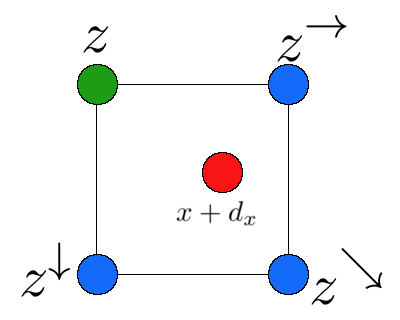
\includegraphics[width=0.5\linewidth]{./images/R1.png}}
    \subfloat[]{\label{fig:region2}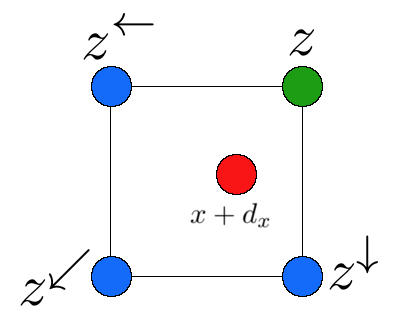
\includegraphics[width=0.5\linewidth]{./images/R2.png}}\\
    \subfloat[]{\label{fig:region2}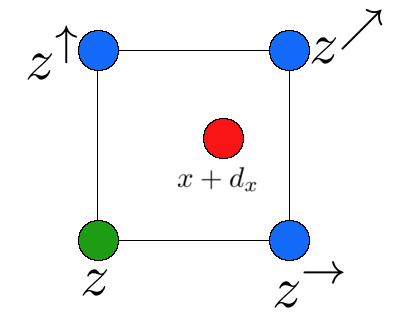
\includegraphics[width=0.5\linewidth]{./images/R3.png}}
    \subfloat[]{\label{fig:region2}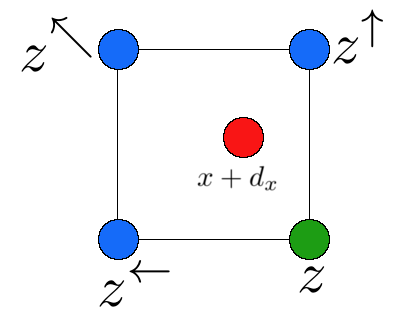
\includegraphics[width=0.5\linewidth]{./images/R4.png}}
    \caption{An input (warped) point $x+d_{x}$ located at regions 1(a),2(b),3(c) and 4(d), with respect to z. The interpolation coefficients can easily be computed as $(\alpha_{x}, \beta_{x})=(1,1)-\lfloor x+d_{x}\rfloor$. }
    \label{fig:dayIndex}
\end{figure}
\end{document}
